\documentclass[a4paper, english, 12pt]{scrartcl}
\usepackage[utf8]{inputenc}
\usepackage[T1]{fontenc}
%\usepackage{babel}
\usepackage{graphicx}
\usepackage{subfigure}
\usepackage[amssymb,binary]{SIunits}
\usepackage{amsmath,amsfonts,amssymb,textcomp,varioref}
\usepackage{verbatim}
\usepackage{times}

%\usepackage[margin=2cm]{geometry}

%\setlength{\parindent}{0 pt}
%\addtolength{\parskip}{\baselineskip}
%\usepackage{setspace}
%\doublespacing

\usepackage{hyperref}

% Set the beginning of a LaTeX document
\begin{document}

\title{Clockless AES circuit}
\author{Kristoffer Ellersgaard Koch}

\date{Fall 2009}
\pagenumbering{roman} % i, ii, iii, iv...
\pagestyle{empty}
\maketitle
\thispagestyle{empty}

\cleardoublepage
\pagestyle{plain}
\thispagestyle{plain}
\section*{Abstract}

Design of digital circuits usually involves a clock. The clock can
however, be one of the greatest contributers to power consumption, and
it is increasingly difficult to distribute a clock over a large
circuit. There exists work on clockless design, and instead use
self-timed techinques to replace the clock. However, theese techniques
are not widely known.

In this project, design of clockless circuits was explored by a
litterature study, and implementation of a clockless Advanced
Encryption Standard (AES) to show the feasability of implementing
reasonable complex clockless circuits. Methods for production testing
were also found.

The result of the study yielded a large AES-module, suggestions for a
workflow for implementing clockless circuits, and pointers to further
research on clockless circuits.

\newpage

\tableofcontents
%\listoffigures


\newpage
\setcounter{page}{1}
\pagenumbering{arabic} % 1, 2, 3...
\section{Introduction}

xxx

\clearpage

\newpage
\section{Theory}

xxx

\clearpage
\newpage
\section{High-level languages and tools}
\label{sec:tools}

To design complex digital circuits, tools for reduction and management
of complexity is needed. Usually, the designer expres the behaviour of
circuits in a hardware description language (HDL), which provides an
abstraction over the underlying hardware. While ordinary design tools
and languages, such as VHDL and Verilog, are not usually used to
synthesize clockless circuits, there is not an inherent limitation in
the languages that prevents this as demonstrated in
\cite[pp. 135-137]{sparso}.

XXX Null convention logic

Most of the work on high-level modeling and synthesis of clockless
circuits is based on the CSP family of languages. The CSP language,
``Communicating Sequential Process'' was proposed by Hoare \cite{csp},
and is based on the mathematical theories of concurrency from process
algebra. CSP-languages allows concurrent processes, composition of
both sequential and parallel statements within a process, and
synchronous message passing between the processes.

\begin{figure}[htbp]
  \centering
  \includegraphics{tangtool.pdf}
  \caption{Tangram design flow. Figure from \cite{fullscan}.}
  \label{fig:tangtool}
\end{figure}

Tangram is a high-level language in the CSP family, designed by
Philips to define clockless circuits. The Tangram compiler generates
what is referred to as handshake circuits, and has its own toolset and
workflow as illustrated in Figure~\ref{fig:tangtool}. Tangram was
later transferred from Philips to the company Handshake Solutions, and
the name of Tangram was changed to Haste. As of this writing, Haste
has entered a state of maintenance, and has been readsorbed into
Philips.

\begin{figure}[htbp]
  \centering
  \includegraphics{handbuffer.pdf}
  \caption{Handshake buffer a) defined in Balsa source code and b)
    implemented as a handshake circuit. Figure from
    \cite{taylor2008automatic}.}
  \label{fig:handbuffer}
\end{figure}

Handshake circuits, as defined in Tangram, consists of 40 different
basic components that can be connected by four-phase handshake
signalling. The components has active and passive ports, where the
active components initiates the handshake and is said to ``push'' the
data. Figure~\ref{fig:handbuffer}.b illustrates a handshake circuit for
a one-place buffer. Active ports are denoted with a filled circle.

There are multiple circuits implemented in Tangram/Haste. XXX list and
explain different circuits.

Balsa is another CSP-like language based on Tangram, and is an attempt
to define a more expressive language. Balsa also introduces a
intermediate file format, breeze, which contains the netlist for the
handshake components. Breeze can later be implemented into
standard-cell logic by. Figure~\ref{fig:balsatool} shows Balsa and
it's related tools.

Tangram and Balsa are referred to as being a ``syntax-directed''
languages. This means that the silicon compiler transparently and
predictably generates components from each language construct. In
Figure~\ref{fig:handbuffer} it is shown how a simple Balsa-program is
translated into a handshake circuit. Each language-construct, loop,
sequence, transfer, and variable, are translated into handshake
components on a one-to-one basis.

Balsa has for example been used to implement two major circuits: The
DMA-controller for the Amulet3a processor, and the ARM-compatible SPA
processor itself. Balsa is released to the public domain under the
GPLv2 licence.

Handshake component based designs has been shown to use little power,
but also to have low performance \cite{80c51}. Handshake-circuits
exhibit a control heavy structure which inhibits performace. Teak
\cite{teak} introduces a new target component set and synthesis scheme
for synthesizing Balsa circuits as an attempt to mitigate this
drawback. Instead of focusing on control

While Balsa-circuits consists of capacity-less channels, where data on
the channel has to be valid from request to acknowledge, Teak allows
buffers to be automatically inserted into the dataflow, allowing
decoupling. 

Teak circuits have been demonstrated to exhibit 4.6\% to 18.39\% worse
performance than Balsa-circuits when syntehsizing to a fixed gate
delay dual-rail four-phase implementation. However, Teak has a larger
headroom for automated optimising transformations.

\subsection{Testing XXX:remove this}


Clockless circuits usually uses latches and C-elements for
memory. These memory-elements are not directly scanable, and they are
not connected to any global clock. However, in \cite{fullscan}, it is
shown how Tangram compiled, clockless circuits can be made scanable by
replacing all state-holding handshake components with scanable
equivalents. In Figure~\ref{scanC}, from \cite{fullscan}, a scanable
C-element is shown. These components are then connected into a serial
scan chain which is compatible with existing ATPG tools.

It is important to note that the scan-chain insertion is done at the
technology-mapping stage, allowing the designer to insert test-logic
into the library of components. For Balsa and Teak, this will require
some modifications of the compilers to chain the memory elements
together into a scan chain, and to provide a global testing clock.

As the testing is done synchronously, it also means that a global
clock have to be implemented. However, this clock has more relaxed
requirements than that of an clocked circuit, since the clock used for
testing runs at lower speeds than the circuit itself is capable of.

\section{new tool}


Languages such as Verilog and VHDL are used to model and simulate
behaviour of digital circuits, and while not all Verilog and VHDL
programs can be synthetizised, a well defined subset can.

Clocked circuits are often expressed in theese languages, but there is
nothing inherent in the languages that prevent a designer from
expressing a clockless circuit. In fact, methods for this have been
used in XXX. However, as shown in \cite[pp XXX]{sparso}, this is
rather cumbersome, and most of the work done on HDLs for clockless
circuits are founded on the programming paradigm introduced with the
language Communicating Sequentaial Processes (CSP)\cite{xxx}, based on
mathematical foundations from process algebra.

As the name partly implies, CSP is baesd on connecting many processes
together whith handshake channels. The most known language based on
CSP is Tangram, designed in 1991 by Philips. Tangram was later split
out to its own company, and changed name to Hast due to trademarking
issues. Haste has now been readsorbed into Philips.

Tangram was used to create multiple circuiots: A XXX microprocessor,
low power smart card XXX, and showed the practical strengths of the
language, design tools,  and clockless circuit design as a
whole.

Tangram emits handshake circuits, first described in
\cite{12,teakxxx}, based on a library of around 40 handshake
components, whith some of theese shown in
figure~\ref{fig:hs}. Figure~\ref{fig:hsbuf} show an one-place buffer
handshake circuit, whith the explicit equest and acknowledge signals
drawn on top. To implement such circuits to hardware, the handshake
components are replaced with their gate-level equivalents, depending
on implementation style. Implementation styles can be bundled data,
QDI, or even clocked for e.g. verification on conventional FPGAs.

Tangram is a so called syntax-directed language, meaning that each
language construct is deterministically mapped to a
handshake-component. This allows the designer to better understand and
optimize circuits as they are written.

To facilitate further research on clockless circuits whithin the
CSP-paradigm, the language ``Balsa'' was designed at Manchester
University \cite{xxx}, and released to the public domain under a GPLv2
license \cite{gpl}. The most complex circuit designed with the balsa
tools, is a clockless ARM\cite{arm} compatible CPU\cite{spa}.

Research have shown that handshake circuits uses little power\cite{xxx},
but also exhibits poor performance\cite{xxx}. Work has been done to
alleviate this\cite{xxx}, but the performance is still rougly half of
clocked equivalents.

To explore and facilitate experiments with automatic optimizations,
and to create more data-flow oriented circuits, ``Teak''\cite{teak}
was recently created, compiling Balsa-programs to a reduced set of 8
different teak-compontents. Teak currently performs worse than the
more mature synthesis tools, but have more room for experimentation
and improvement at the compiler level.



\clearpage
\newpage


\section{The Advanced Encryption Standard (AES)}

On September 12, 1997, the United States' National Institute of
Standards and Technology (NIST) announced an open competition to
develop a new symmetric-key block cipher algorithm to replace the
ageing DES (Data Encryption Standard). The demands was that the AES
should be an unclassified, public, and royalty-free symmetric-key
encryption algorithm supporting block sizes of 128-bits, key sizes of
128-, 192- and 256-bits.

On October 2, 2000, NIST announced that it had selected
Rijandael~\cite{rijandael}, designed by two Belgium cryptographers:
Daemen and Rijmen, as the AES.

%As of today, multiple processors include native support for
%acceleration of AES-specific operations. NIST has also called for the
%development of a new hash-function, and 4 of 14 of the remaining
%candidates rely on native AES-acceleration to acheive performance.

\subsection{Overview of the algorithm}

Rijandael is a symmetric-key block-cipher algorithm. This means that
encryption is defined as $c \leftarrow E_k(m)$, and decryption as $m
\leftarrow D_k(c)$, given a key $k$, a message $m$ and a ciphertext
$c$. Rijandael supports variouskey sizes, but I will confine the
description and implementation to a key size to
\unit{128}{\bit}. This will not cause a big loss of generality to the
working principle. I will also limit the implementation to
encryption-only.

The Rijandael cipher segments a 128-bit message into 16 bytes,
represented by a $4 \times 4$ matrix:

\begin{equation}
  m = \begin{pmatrix}
    m_0 & m_4 & m_8 & m_{12} \\
    m_1 & m_5 & m_9 & m_{13} \\
    m_2 & m_6 & m_{10} & m_{14} \\
    m_3 & m_7 & m_{11} & m_{15}
    \end{pmatrix}
\end{equation}

This is referred to as the $State$ throughout the algorithm, and it is
permutated 10 $Round$s in the algorithm. For larger key sizes, the
number of rounds should be increased. A round is composed of four
transformations described below:

\begin{eqnarray*}
&Round&(State, RoundKey) \{\\
  & &SubBytes (State)\\
  & &ShiftRows (State)\\
  & &MixColumns (State)\\
  & &AddRoundKey (State, RoundKey)\\
&\}&
\end{eqnarray*}

The final round, $FinalRound$, is slightly different: it excludes the
MixColumns stage. $RoundKey$ is derived from the key by the key
expansion scheme also described below. For decrypting, given the
correct key, there exists inverse functions for each round.

The Rijandael cipher work in a finite field. The field is realized as
all polynomials modulo the irreductible polynomial 
\begin{equation}
  f(x) = x^8 + x^4 + x^3 + x + 1
  \label{eq:gf}
\end{equation} 
over $\mathbb{F}_2$. This is called the ``Rijandael
field'', and $\mathbb{F}_{2^8}$ is often used to denote the field with
256 elements.

Each element can also uniquely be represented as a 8-bit byte, $\{b_7
b_6 b_5 b_4 b_3 b_2 b_1 b_0\}$ yielding the polynomial $\sum_{i=0}^7
b_i x^i$, where $b_i \in \mathbb{F}_2$ where $\mathbb{F}_2 =
\{0,1\}$. The polynomial $x^2 + 1$ can thereby be represented as
$\{00000101\}$, or hexadecimaly as $\{05\}$.  All operations on
elements in this field results in an element within the field. The
field supports addition and multiplication between two field elements.

The $SubBytes$ routing subtitutes all bytes using $y = A x^{-1} + b$.
%%  where $
%%   A =
%%   \begin{pmatrix}
%%     1 & 0 & 0 & 0 & 1 & 1 & 1 & 1 \\
%%     1 & 1 & 0 & 0 & 0 & 1 & 1 & 1 \\
%%     1 & 1 & 1 & 0 & 0 & 0 & 1 & 1 \\
%%     1 & 1 & 1 & 1 & 0 & 0 & 0 & 1 \\
%%     1 & 1 & 1 & 1 & 1 & 0 & 0 & 0 \\
%%     0 & 1 & 1 & 1 & 1 & 1 & 0 & 0 \\
%%     0 & 0 & 1 & 1 & 1 & 1 & 1 & 0 \\
%%     0 & 0 & 0 & 1 & 1 & 1 & 1 & 1
%%   \end{pmatrix}$ and $
%%   b = 
%%   \begin{pmatrix}
%%     1\\1\\0\\0\\0\\1\\1\\0
%%   \end{pmatrix}$.
That is, inversion in the finite galois field, followed by a short
linear transformation.

$ShiftRows$ is a permutation of the order of the bytes in the state:
\begin{equation}
  \begin{pmatrix}
    s_0 & s_4 & s_8    & s_{12} \\
    s_1 & s_5 & s_9    & s_{13} \\
    s_2 & s_6 & s_{10} & s_{14} \\
    s_3 & s_7 & s_{11} & s_{15}
  \end{pmatrix} 
  \rightarrow
  \begin{pmatrix}
    s_0    & s_4    & s_8    & s_{12} \\
    s_{13} & s_1    & s_5    & s_9 \\
    s_{10} & s_{14} & s_2    & s_6 \\
    s_7    & s_{11} & s_{15} & s_3    
    \end{pmatrix}
\end{equation}
In VLSI circuits, this is easily implemented as wiring.

The $MixColumn$ procedure scrambles all the columns in the state
%given as $
%\begin{pmatrix}
%  s_0\\s_1\\s_2\\s_3
%\end{pmatrix}$, 
by multiplying them with the matrix
\begin{equation}
  \begin{pmatrix}
    \{02\} & \{03\} & \{01\} & \{01\} \\
    \{01\} & \{02\} & \{03\} & \{01\} \\
    \{01\} & \{01\} & \{02\} & \{03\} \\
    \{03\} & \{01\} & \{01\} & \{02\}
  \end{pmatrix}
  \label{eq:mixcol}
\end{equation}
in the galois field. Multiplication, $q(x)=a(x) \otimes b(x)$, in the
galois field is multiplication of two polonomials modulo the
irreductible polinomial \eqref{eq:gf}. The multiplication can be
performed by generating up to eight partial products
\begin{equation}
  P_i(x) = a(x) x^i
\end{equation}
iterativly as 
\begin{equation} 
  P_i = 
  \begin{cases}
    a(x) & \text{if} \quad i = 0 \\
    x P_{i-1}(x) & \text{if} \quad i > 0
  \end{cases}
  \label{eq:gfdouble}
\end{equation}
and then adding the partial products according to the bits $b_i$ in
$b(x)$, yielding the result as
\begin{equation}
  q(x) = \sum_{i=0}^{7} P_i(x) b_i
  \label{eq:addpart}
\end{equation}
. Note that the $\sum$ here performs the additions in the Galois
field, i.e. it sums with xor. Each iteration with $i > 0$ in
\eqref{eq:gfdouble} can be seen as a ``doubling'' in the galois field,
making the multiplication an analogy to peasant's multiplication in
\eqref{eq:addpart}. The ``doubling'' can be implemented with a shift
and 3 xor gates.

$AddRoundKey$ performs simple addition of the expanded key and the
state in the galois field. This addition can be implemented by simple
xor. The expanded key, derived from the input key, is calculated by
operations similar to the round function, and needs 4 bytes of
$SubBytes$ transformation as well.

\subsection{Performance of the AES}

As a reference of the relative performance of the AES, a simple
benchmark was done on a computer\footnote{openssl version
  0.9.8g. Measurement performed with the command ``openssl time
  aes''.}. The results are shown in table~\ref{tab:aes}. A feasability
study \cite{feas} shows that throughput up to \unit{500}{\giga \bit
  \per \second} should be possible on VLSI.

\begin{table}[h]
  \centering
  \begin{tabular}{|c|c|}
    \hline
    \emph{Key size}  & \emph{Throughput} \\ \hline
    \unit{128}{\bit} & \unit{111}{\mega \byte \per \second} \\
    \unit{192}{\bit} & \unit{94.7}{\mega \byte \per \second} \\
    \unit{256}{\bit} & \unit{82.3}{\mega \byte \per \second} \\ \hline
  \end{tabular}
  \caption{Performance of AES on an Intel Pentium 4 2.8 GHz CPU.}
  \label{tab:aes}
\end{table}

The clockless AES module designed in \cite{claes}, which did not have
performance as a primary objective, performed \unit{283.75}{\kilo
  \byte \per \second} on \unit{0.35}{\micro \meter} CMOS.

\subsection{Details for VLSI implementation}

When implementing AES to hardware, there are a lot of choices and
optimizations that can be applied. I will here outline some aspects of
implementing AES. More methods for saving power and enhancing
performance are rigourously surveyed in \cite{ekelund}.

Naivly, the $SubBytes$ routine and its inverse is implemented with a
table lookup with 256 entries. In hardware, this means some kind of a
ROM, with an unbreakable latency and the inherent impossibility for
pipelining. In \cite{csbox} a method is described for decomposing the
$2^8$ fields into smaller $2^4$ fields for calculating the
multiplicative inverse combinationally.

The AES algorithm in itself is considered a secure cipher, that is, no
other methods other than brute-force attacks exists to deduce a key or
plaintext. However, an implementation of AES in software or hardware
can be subject to side-band attacks. If an attacker has physical
access to a weak system performing AES, multiple techniques exists for
retrieving information about the key.

If not carefully implemented, a circuit can exhibit non-constant
timing when performing, revealing patterns of the data being
processed, that being the key or plaintext. Implementations can also
have weaknesses where the power dissipation depends on the data, which
lets a careful attacker measure and gather data about the key. A third
method is to inject faults into a system, making it malfunction and
reveal secret data.

The clockless AES implemented in \cite{claes} was developed to avoid
these kind of attacks, and concludes that their dual-rail
implementation hides the secret data from power, timing and
fault-injection attacks. It is worth to note that the ROM-based
implementation of $SubBytes$ that was utilized in this implementation
showed major leaks of information in the circuit. Side-band
information is leaked as a consequence of different hamming-weights
are giving different power signatures, and this problem is alleviated
in \cite{claes} by employing dual-rail encoding, ensuring constant
hamming-weight at the electrical level for all data.

\subsection{Pipelining and mode of operation}

While it is possible to pipeline the $Round$ procedure by itself, and
even $SubBytes$ itself when implemented combinationally as in
\cite{csbox}, it can also be beneficial to unroll multiple $Round$s in
series. I will here describe 3 modes of operation to illustrate when
unrolling can be beneficial.

\begin{figure}[htbb]
  \subfigure{\label{fig:ecbpicta}}
  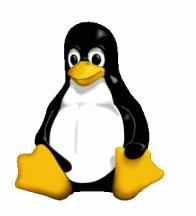
\includegraphics[width=0.3\textwidth]{tux.jpeg}
  \subfigure{\label{fig:ecbpictb}}
  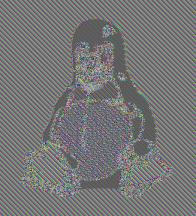
\includegraphics[width=0.3\textwidth]{tux_ecb.jpeg}
  \subfigure{\label{fig:ecbpictc}}
  
\includegraphics[width=0.3\textwidth]{noise.png}
  \caption{a) A picture encrypted in b) ECB-mode and in c) other
    modes, causing an unrevealing pseudo random pattern. Figure from
    \cite{pingu}.}
  \label{fig:ecbpict}
\end{figure}

When encrypting a plaintext with a length over 128 bits, the most
straightforward way is to split the plaintext into 128-bit blocks and
encrypt them individually. This is called the electronic codebook mode
of operation, or ECB. As the blocks can be encrypted and decrypted
independently, this method allows pipelining with unrolled
$Round$s. However, as the AES-algorithm deterministicly yields the
same output given the same input (key and data), it allows an attacker
to guess the ciphertext by trial-and-error. Figure~\ref{fig:ecbpict}
illustrates how ECB reveals data-patterns from the plaintext.


\begin{figure}[htbb]
  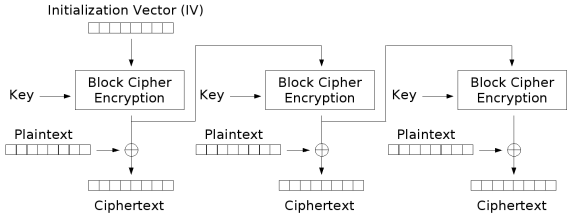
\includegraphics{ofb.png}
  \caption{Output feedback (OFB) mode encryption. Figure from \cite{pingu}.}
  \label{fig:ofb}
\end{figure}

The output feedback (OFB\nomenclature{OFB}{Output Feedback}) mode of
operation, described in figure~\ref{fig:ofb}, while not suffering from
the same weakness as the ECB\nomenclature{ECB}{Electronic Code Book}
mode, does not benefit from unrolling, as the preceeding ciphertext is
needed to encrypt the current plaintext. The OFB mode generates a
pseudo random (but unguessable, not given the key) string that is
XORed\nomenclature{XOR}{Exclusive OR} with the plaintext to encrypt,
similar to the Vernam one-time-pad cipher \cite{vernam}.

The only mode of operation considered secure, to my knowledge, that
benefit from loop unrolling, is the counter
(CTR)\nomenclature{CTR}{Counter} mode. In this mode, similar to the
OFB mode, a pseudorandom string is generated simpy by encrypting an
integer, $i$, corresponding to the current block number, that is $c_i
= m_i \oplus E_k(i)$, and similary $m_i = c_i \oplus E_k(i)$, where
$\oplus$ denotes XOR. Whithout feedback, the CTR mode allows random
access during encryption and decryption (for e.g. full disk
encryption), and blocks can be processed in paralell.

\subsection{Decryption and other keysizes}

While this project does not cover decryption and the larger keysizes,
that is 192 and 256 bit, I will shortly outline how this can be
implemented, and roughly estimate the impact on area and performance
it will inflict.

The decryption is rougly the algorithms performed inversely with
reverse operations for $SubBytes$, $ShiftRows$, $MixColumns$ and
$AddKey$: 
\begin{itemize}
  \item $SubBytes^{-1}$, implemented combinational, is the same
    operation as $SubBytes$, except for the relativily short linear
    transform, which needs an inverse.
  \item $ShiftRows^{-1}$ has, like $ShiftRows$, the simplest
    implementation as wires. 
  \item $MixColumns^{-1}$ uses different and larger coefficients
    than $MixColumns$ \eqref{eq:mixcol}, demanding 2 more partial
    products \eqref{eq:gfdouble} to be calculated in the
    galois field multiplications, and thereby causing longer
    delays. The calculation of the partial products can be shared
    between $MixColumns$ and its inverses. 
  \item $AddRoundKey^{-1}$ can use the same hardware as
    $AddRoundKey$. 
\end{itemize}
The keyschedule for the decryption is the same as for encryption.

Expanding the algorithm to key sizes of 192 and 256 bit requires
expansion of the key registers and changes to the control logic and
the key schedule. The control logic must be changed, as 128, 192, and
256 bit keys respectivily requires 10, 12, and 14 $Round$s to be
performed. The key schedule also demands an extension of the control
logic to support the larger key sizes.

Implementing decryption alongside with encryption will, as discussed
above, have negative effect on the performance, as there will be a
greater control overhead. The area will also increase, but as most of
the operations can be generalized to also provide an inverse, the area
overhead should not be dramatic. Expansion of the supported key sizes,
in addition to the obvious demand of larger registers, only requires
minor expansion of the control logic.

\clearpage
\newpage

\section{Implementation of clockless AES}

The AES was written in Balsa in a way that support both Balsa and
Teak simulation and synthesis, avoiding incompatibilites. Focus was at
producing a correct implementation before performance and power, to
demonstrate the feasability of using the tools for relativly
large-scale implementations.

The AES was implemented in an architecture with four 128-bit
registers, two for the data, and two for the key and
key-expansion. Two registers is needed for each, as they are
implemented as single latches and not master/slave latches which does
not, by design, support auto assignments of the form 
$var := var + 1$. The architecture was designed with one control-input,
$instruction$ and two 32-bit data-ports; one for input and one for
output. Seven instructions was defined to load, permutate and unload
data from the 128-bit key AES-encryption-circuit:

\begin{description}
  \item[load\_data] Loads 4 32-bit words of data into $reg_0$.
  \item[load\_key128] Loads 4 32-bit words of key into $key_0$.
  \item[add\_key] Sets $reg_1 := reg_0 xor key_0$ (addition in the
    galois field) and then sets $reg_0 := reg_1$ and $key_1 := key_0$.
  \item[sub\_bytes] Calculates $reg_1 := SubBytes(ShiftRows(reg_0))$.
  \item[mix\_col\_expand] Calculates $reg_0 := MixColumns(reg_1)$, and
    $key_0 := ExpandKey(key_1)$.
  \item[skip\_mix\_expand] Only calculates $key_0 := ExpandKey(key_1)$.
  \item[output\_data] Outputs data in $reg_0$ as 4 32-bit words.
\end{description}

To facilitate the testbench, the module aes\_ctrl issues instructions
to the data-path module aes\_data. The source code and corresponding
breeze handshake circuit is shown in figure~\ref{fig:aesctrl}. The
sequence of instructions from aes\_ctrl causes key and plaintext to be
loaded through the input port, encrypted, and then emitted through the
output port. The sourcecode is also shown to illustrate the
straightforwardness of defining sequential behaviour in Balsa and
similar languages.

\begin{figure}[htbp]
  \centering
  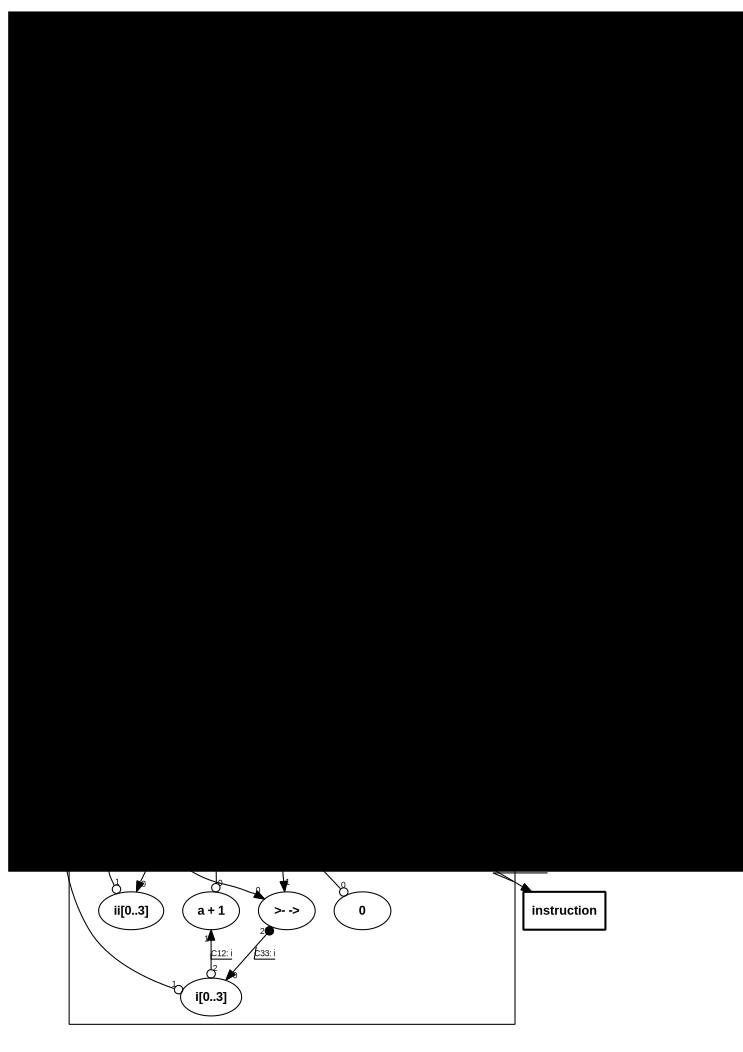
\includegraphics[height=0.9\textheight]{aesctrl.pdf}
  \caption{Source code for AES control module and Balsa handshake
    implementation.}
  \label{fig:aesctrl}
\end{figure}

Most of the instructions operate on 32-bit blocks in series, with the
exception of ``add\_key'', which adds all the 128 bits in one
chunk. 32 bit was chosen, as this is the size of a column, and
choosing a smaller datapath would complicate the $MixColumn$
stage. Results from \cite{ekelund} also showed that processing 32 bits
at the time is favorable.

The ``instruction'' architecture was choosen to ease debugging, and
hurts the performance, as it delays the execution of $MixColumn$,
which can be performed on the data returned from the $SubBytes$
stage. The order of $ShiftRows$ and $SubBytes$ have been reversed, as
this was most practical in the implementation, and does not hurt
correctnes.

The $SubBytes$-module was implemented directly from the architecture
given in \cite{xxxcsbox}.

The resources used in the top level design is:
\begin{itemize}
   \item 4 8-bit combinational SubBytes circuits, as as described in
     \cite{combsbox}, shared between the datapath and the keypath.
   \item 1 32-bit mixcolumn circuit employing XXX ``doublers''
   \item 1 128-bit xor-adder circuit
   \item 1 galois field ``doubler'' for the key schedule.
\end{itemize}

The design was designed in Balsa, with frequent compilations to
handshake circuits to visualize what kind of circuit that was
generated. Validation under development was performed using the
behaviroal simulation tool in Balsa, breeze-sim, simulating the
behaviour of the Breeze handshake circuits. Each sub-module was
verified for itself, sub-bytes and gfdouble exhaustivly, checking each
of the 256 input output value pairs. The complete AES module was
verified using the NIST ECB testing vectors \cite{nisttest}.

\begin{figure}[htbp]
  \centering
  \includegraphics{teaklib.pdf}
  \caption{Library compontents used to synthesize netlists from Balsa
    code with Teak. Combinations omitted in truth tables signifies
    that state is kept.}
  \label{fig:teaklib}
\end{figure}

While it should be able to implement the breeze handshake circuits to
functionally equivalent netlists for mapping to hardware, I was not
able to do this with the latest version of Balsa\footnote{Balsa 4.0,
  as of this writing, not publicly available, kindly supplied by XXX
  at Manchester University.}, due to missing library files and
documentation. For implementation, I concentrated on using Teak
\cite{teak}, producing netlists consisting of constant delay gates as
shown in figure~\ref{fig:teaklib}.

In addition to the behavrioal simulation, the Verilog netlist
generated from Teak was verified using the GPL version of the verilog
simulation tool cver using the 4 first test-vectors used in the
behavioural simulation, limited by instability of the simulation tool.

\clearpage
\newpage
\section{Results and Discussion}

The emphasis of this project was not the AES module itself, but the
workflow outlined for specifying behaviour at a high level, and
obtaining a netlist correctly implementing the specified
behaviour.

\begin{table}[h]
  \centering
  \begin{tabular}{|c|c|}
    \hline
    \emph{Component}  & \emph{Count} \\ \hline
    AND2 & 8493 \\
    AND3 & 2 \\
    NAND2 & 501 \\
    NAND3 & 146 \\
    OR2 & 3982 \\
    OR3 & 39 \\
    NOR2 & 785 \\ 
    NOR3 & 1517 \\
    BUFF & 4131 \\
    INV & 560 \\
    AO22 & 692 \\
    AO222 & 8 \\
    C2 & 2609 \\
    C2R & 1093 \\
    C3  & 2130 \\
    AC2 & 0 \\
    \hline
  \end{tabular}
  \caption{Resource usage in terms of gates listed in
    figure~\ref{fig:teaklib} on page~\pageref{fig:teaklib}}
  \label{tab:res}
\end{table}

The Verilog netlist generated by Teak from the Balsa sourceode
contained 65421 lines. This also includes the test-bench enclosure,
inputting one key and plaintext, and printing the
ciphertext. Table~\ref{tab:res} summarizes the resource usage of the
Teak circuit, with the primitives illustrated in
figure~\ref{fig:teaklib} on page~\pageref{fig:teaklib}.

The performance was not measured, as this was a non-trivial procedure
with the choosen verilog simulator, which also prooved itself quite
unstable given the large verilog netlist. The litterature suggests
that my choices would yield a poorly performing circuit, as Teak has
been shown to currently perform worse than Balsa, which in turn
performs worse than conventional clocked circuits.

However, clockless circuits have other properties than clocked
circuits, which can be important for applications where performance is
not the primary objective. Low power is no longer considered a niche,
and as shown in \cite{claes}, clockless circuits can have good
characteristics with for secure implemetation of crypto algorithms.

It is also interesting how much effort that went into producing a
working AES module. I did not keep track of how many hours that went
into learning the Balsa language, or to write the AES, but after
understanding the basic handshake mechanisms, writing working Balsa
programs was quite straighforward. CSP languages, as noted in
\cite{taylor}, allows specifications to be expressed in way that is
similar to programmers accustomed to imperative programming languages,
such as C, lowering the threshold for doing hardware design, ``even
for novices''. While specifications written in CSP style languages
such as Balsa and Tangram are not guaranteed to be efficiently
implemented, tools such as visual simulators allows the designer to
gain a better understanding of how the design performs, find
bottlenecks and to optimize the sourcecode when required.

While low area and high performance are often cited goals for a
digital circuit specification, the time consumed by engineers to
design and verify a circuit is also important. If a design meets the
required constraints, e.g. it meet its realtime deadlies, and the
design fits on a specified FPGA, no further optimizations should be
required.

While I was able to develop an AES with the available tools, I
encountered bugs on many occasions, which I sometimes was not able to
work around. The most important problem was a compiler bug in Balsa
3.5.1, which prevented compilation of my AES module. I was later
supplied with the newest Balsa 4.0 which was able to generate
handshake circuits in the Breeze-format, but not able to further
generate netlists. While this illustrates that the choosen tools are
currently a bit immature, they are under development, and are expected
to improve.


\clearpage
\newpage
\section{Conclusion and further work}

xxx

Bonus: Cite buitiful Dijikstra.


\clearpage
\newpage
\appendix

%\section{Source code}

All listed source code is also available at
http://github.com/kristofferkoch/naive-AES-balsa.

\subsection{Test fixture, test-simple.balsa}

The input is automatically inserted by a script to test series of
vectors. First 4 32-bit words are key, last words are plaintext. All
data are most significant data first, that is leftmost state-column
first.

\lstinputlisting{naive-AES-balsa/test-simple.balsa}

\subsection{aes.balsa}
\lstinputlisting{naive-AES-balsa/aes.balsa}

\subsection{sbox.balsa}
\lstinputlisting{naive-AES-balsa/sbox.balsa}

\subsubsection{affine.balsa}
\lstinputlisting{naive-AES-balsa/affine.balsa}

\subsubsection{inversion.balsa}
\lstinputlisting{naive-AES-balsa/inversion.balsa}

\subsubsection{gf4.balsa}
\lstinputlisting{naive-AES-balsa/gf4.balsa}


\subsection{mixcolumn.balsa}
\lstinputlisting{naive-AES-balsa/mixcolumn.balsa}

\subsection{gfdouble.balsa}
\lstinputlisting{naive-AES-balsa/gfdouble.balsa}

%\clearpage
%\newpage

%\input{fremdriftsplan}
%\clearpage
%\newpage

%\newpage
\label{ssec:littref}
\bibliography{boker} 
\bibliographystyle{plain}


\end{document}

